\chapter{Conexões entre neurônios}\label{cap:conexoes}
\section{Introdução}\label{sec:conexoes_intro}
Uma vez visto o comportamento de um neurônio individualmente, este Capítulo traz informações sobre como se dá a conexão entre neurônios.
%TODO: melhorar
\section{Sinapses}\label{sec:sinapses}
A sinapse é uma conexão entre dois neurônios. Elas podem ser elétricas, que se dão a partir de uma junção entre as duas células, por onde íons podem passar, produzindo uma corrente sináptica proporcional à diferença entre os potenciais de membrana das duas células, ou químicas, que são conectadas através de um espaço entre as células, e a interação entre elas se dá pela liberação de neurotransmissores, que é um elemento químico que se propaga nesse espaço, fazendo a comunicação entre eles. As sinapses químicas são majoritárias no cérebro humano pós-natal, enquanto que as elétricas estão presentes em quantidade relevante apenas durante o período de desenvolvimento embrionário humano. As sinapses químicas são categorizadas em excitatórias ou inibitórias, de acordo com o efeito no potencial de membrana da célula pós-sináptica (a que responde à liberação do neurotransmissor após o potencial de ação do neurônio pré-sináptico). Enquanto as sinapses excitatórias despolarizam a membrana, as inibitórias causam hiperpolarização, facilitando ou dificultando, respectivamente, o potencial de ação da célula pós-sináptica. Os neurotransmissores mais comuns associados aos neurônios corticais são o \textbf{glutamato}, que excita a célula pós-sináptica, e o \textbf{ácido $\gamma$-aminobutírico (GABA)}, que a inibe.
%TODO: acrescentar nota de rodapé sobre o gaba ser excitatório em algumas condições (dentro do útero materno, por exemplo)
O esquema de uma sinapse química é mostrado na Figura~\ref{fig:sinapses}. Os neurotransmissores são transportados por compartimentos ao redor da membrana neuronal chamados de vesículas.
\begin{figure}[tb]
	\centering
	\caption{Esquema simplificado de uma sinapse química}
	\label{fig:sinapses}
	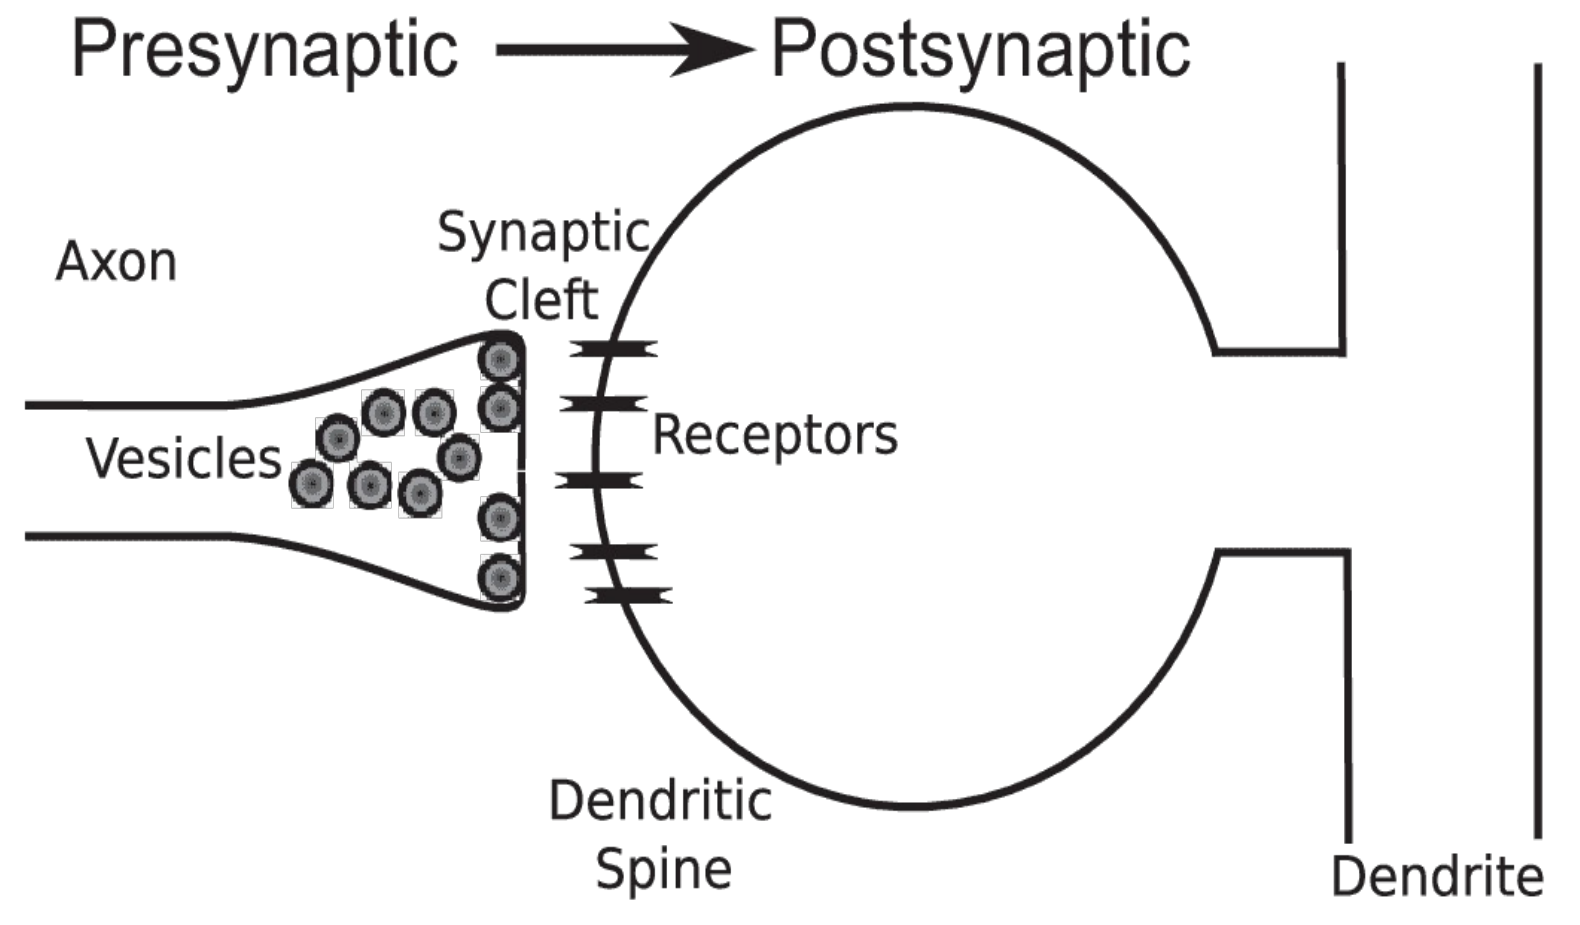
\includegraphics[width=0.7\linewidth]{figs/sinapses}\\
	\small{Fonte: \cite{miller_introductory_2018}}
	%TODO: trocar figura
\end{figure}

A transmissão sináptica é modelada usando a equação abaixo \cite{dayan_theoretical_2001}:
\begin{equation}\label{eq:sinapse}
	\frac{dG_{sin}(t)}{dt}=\frac{-G_{sin}(t)}{\tau_{sin}}
\end{equation}
sendo $G_{sin}(t)$ a condutância sináptica e $\tau_{sin}$ a constante de tempo específica para o tipo de sinapse. Além disso, se houver disparo da célula pré-sináptica, ocorre o seguinte mapeamento:
\begin{equation}\label{eq:sinapse_mapeamento}
	G_{sin}(t)\mapsto G_{sin}(t)+\Delta G
\end{equation}
onde $\Delta G$ é o incremento de condutância. Um modelo mais elaborado considera o crescimento e decaimento de condutância usando a equação abaixo \cite{miller_introductory_2018}:
\begin{equation}\label{eq:sinapse_delta}
	\Delta G_{sin}(t)=\frac{\Delta G}{K}e^{-(t-t_{disparo})/\tau_{decai}}\Big[1-e^{-(t-t_{disparo})/\tau_{cresce}}\Big]
\end{equation}
com $\tau_{cresce}$ a constante de crescimento, $\tau_{decai}$ a de decaimento ($\tau_{decai}>\tau_{cresce}$), $t_{disparo}$ o instante do disparo da célula pré-sináptica, e $K$ um fator para garantir que a condutância tenha um valor máximo igual a $\Delta G$, calculado por:
\begin{equation}\label{eq:sinapse_k}
	K=\Bigg(\frac{\tau_{decai}}{\tau_{cresce}+\tau_{decai}}\Bigg)\Bigg(\frac{\tau_{cresce}}{\tau_{cresce}+\tau_{decai}}\Bigg)^{\tau_{cresce}/\tau_{decai}}
\end{equation}
A dinâmica da condutância sináptica é mostrada na Figura~\ref{fig:respostasinaptica}, onde é possível observar o incremento da condutância sináptica (curva de cima) após a ocorrência de um potencial de ação (linhas verticais do gráfico embaixo).

\begin{figure}[tb]
	\centering
	\caption{Condutância sináptica em resposta aos potenciais de ação da célula pré-sináptica}
	\label{fig:respostasinaptica}
	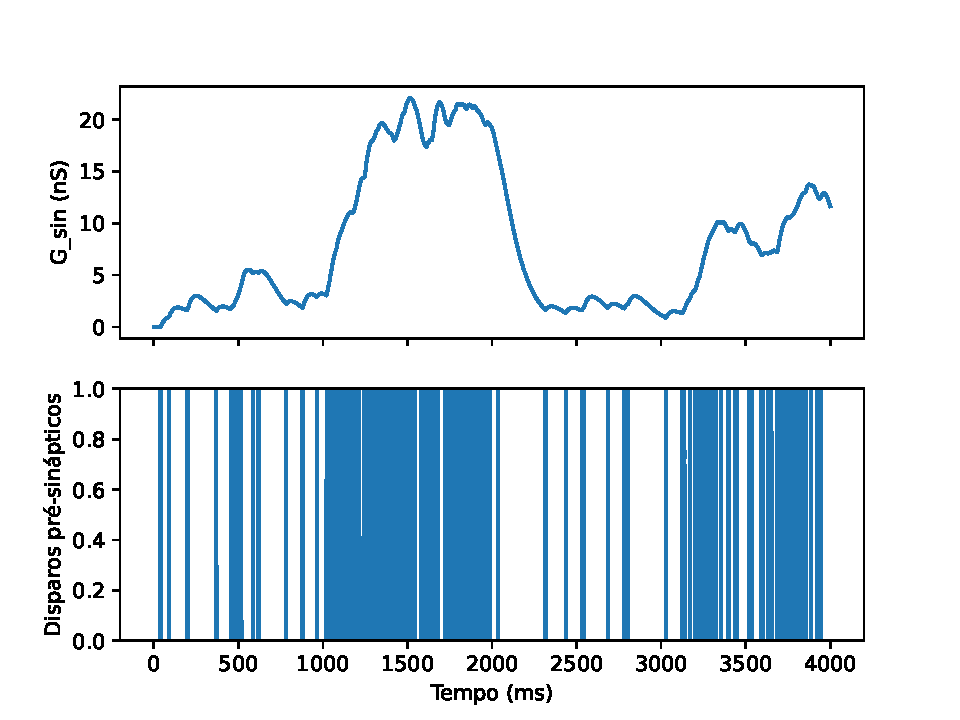
\includegraphics[width=0.7\linewidth]{figs/resposta_sinaptica}
	%TODO: regerar
\end{figure}

\subsection{Sinapses dinâmicas}\label{subsec:sinapses_dinamicas}
Acima, os modelos de sinapses possuem pesos fixos. Entretanto, fisiologicamente, as condutâncias sinápticas não são fixas, mas mudam de acordo com a disponibilidade de recursos sinápticos no terminal pré-sináptico, determinados por algumas condições de entrada. Esse comportamento é chamado de sinapse dinâmica, cuja força da conexão varia em um curto período de tempo, ocasionando o a chamada plasticidade de curto prazo (ou de curta duração). Experimentalmente, são observados dois tipos, com efeitos opostos na eficácia sináptica, como mostrados na Figura~\ref{fig:plasticidadecurtaduracao}. À esquerda, é exibido o fenômeno da depressão de curta duração, que causa uma redução temporária na força sináptica, e à direita o fenômeno da facilitação de curta duração, que causa um incremento temporário.
\begin{figure}[tb]
	\centering
	\caption[Depressão e facilitação sináptica]{Depressão e facilitação sináptica}
	\label{fig:plasticidadecurtaduracao}
	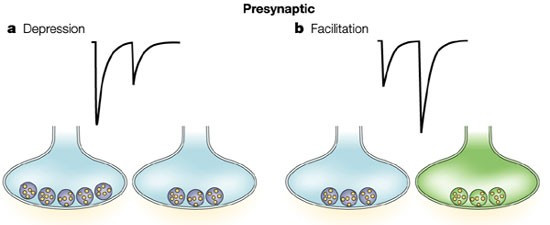
\includegraphics[width=0.7\linewidth]{figs/plasticidade_curta_duracao}
	%TODO: trocar figura
\end{figure}
O modelo matemático da PCP é fundamentado no conceito de uma quantidade limitada de recursos sinápticos disponíveis para transmissão, tal como a quantidade total de vesículas sinápticas. Esse número de recursos pré-sinápticos muda dinamicamente de acordo com o histórico recente de picos de atividade. Após um pico pré-sináptico, a probabilidade de liberação do conjunto disponível para utilização aumenta devido ao influxo de cálcio induzido pelo pico no terminal pré-sináptico. A simulação de depressão e facilitação sinápticas pode ser feita alterando-se o valor de $\Delta G$ acima para:
\begin{equation}\label{eq:sinapse_facilitacao_depressao}
	\Delta G=G_{max}p_0FD
\end{equation}
com $G_{max}$ o valor máximo de condutância sináptica, $p_0$ a probabilidade de liberação do neurotransmissor, e $F$ e $D$ as variáveis de facilitação e depressão sináptica, atualizadas por:
\begin{equation}\label{eq:depressao_sinaptica}
	\frac{dD}{dt}=\frac{1-D}{\tau_D}
\end{equation}
\begin{equation}\label{eq:facilitacao_sinaptica}
	\frac{dF}{dt}=\frac{1-F}{\tau_F}
\end{equation}
e, seguindo cada disparo da célula pré-sináptica, ocorrem os seguintes mapeamentos:
\begin{equation}\label{eq:mapeamento_depressao_sinaptica}
	D\mapsto D-p_0FD
\end{equation}
\begin{equation}\label{eq:mapeamento_facilitacao_sinaptica}
	F\mapsto F+f_{fat}(F_{max}-F)
\end{equation}
com $F_{fat}$ denotando o grau de facilitação ($0\leq f_{fat}\leq 1$) e $F_{max}$ o seu valor máximo.

%% falar da bomba de sódio e potassio ao falar do potencial de membrana

\section{Multi-estabilidade}\label{sec:biestabilidade}

\subsection{Oscilações e multi-estabilidade}
Além das alterações de comportamento causadas pelas entradas aplicadas (injeção de corrente), os neurônios podem mudar sua resposta de acordo com as conexões feitas uns com os outros. A capacidade dos neurônios de manter múltiplos estados de atividades mesmo recebendo valores idênticos de entrada é chamada de \textbf{multi-estabilidade}. O próprio neurônio de Hodgkin-Huxley, visto anterior, podes alternar entre um estado de quiescência, exibindo oscilações sub-limiares (variações no potencial de membrana insuficientes para a produção de um potencial de ação), e um estado de ressonância, que é uma resposta recorrente, conforme mostrado na Figura~\ref{fig:hhdinamico}. Nos três cenários é aplicado um pulso de corrente no intervalo de $0,05$ até $0,45\ s$, porém variando a amplitude. É possível observar que, para $0,300\ nA$ (no topo) ocorre apenas um disparo de potencial de ação, com uma oscilação em seguida. Para $0,624\ nA$ (no meio), alguns disparos acontecem, porém não o suficiente para ativar o comportamento ressonante, que é conseguido com um leve incremento de corrente, para $0,626\ nA$ (embaixo).

\begin{figure}[tb]
	\centering
	\caption{Comportamento variado do modelo de Hodgkin-Huxley para diferentes correntes}
	\label{fig:hhdinamico}
	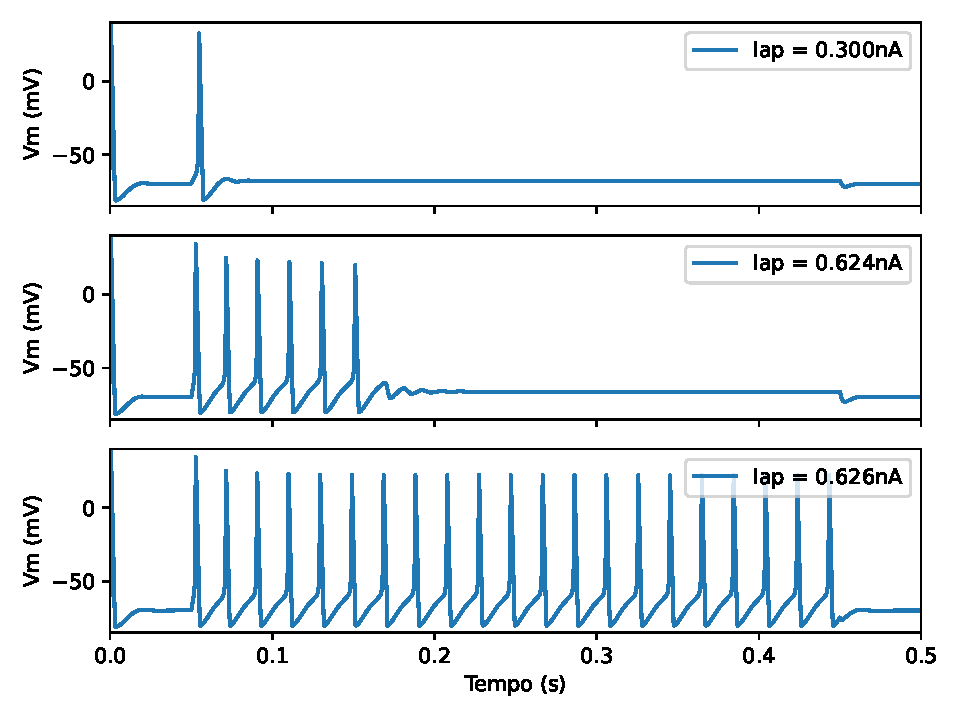
\includegraphics[width=0.7\linewidth]{figs/hh_dinamico}
	%TODO: regerar
\end{figure}
A forma mais simples de multi-estabilidade é a bi-estabilidade, onde, com um mesmo estímulo, dois estados de atividade neuronal podem ocorrer, gerando a chamada rivalidade perceptual, onde estímulos únicos podem ser percebidos de mais de uma maneira, alterando entre cada um dos perceptos (percepções bi-estáveis), como nos exemplos da Figura~\ref{fig:biestabilidade}. Na Figura~\ref{fig:cubonecker}, o cubo pode ser visto com a face frontal em lugares diferentes. Já na Figura~\ref{fig:cao_homem}, ora a imagem aparenta ser um cachorro visto de frente, ora parece um homem de costas.

\begin{figure}[tb]
	\centering
	\caption{Imagens produzindo percepções de bi-estabilidade}
	\label{fig:biestabilidade}
	\begin{subfigure}[]{0.3\textwidth}
		\caption{O cubo de Necker pode ser visto com a face frontal em lugares diferentes}
		\label{fig:cubonecker}
		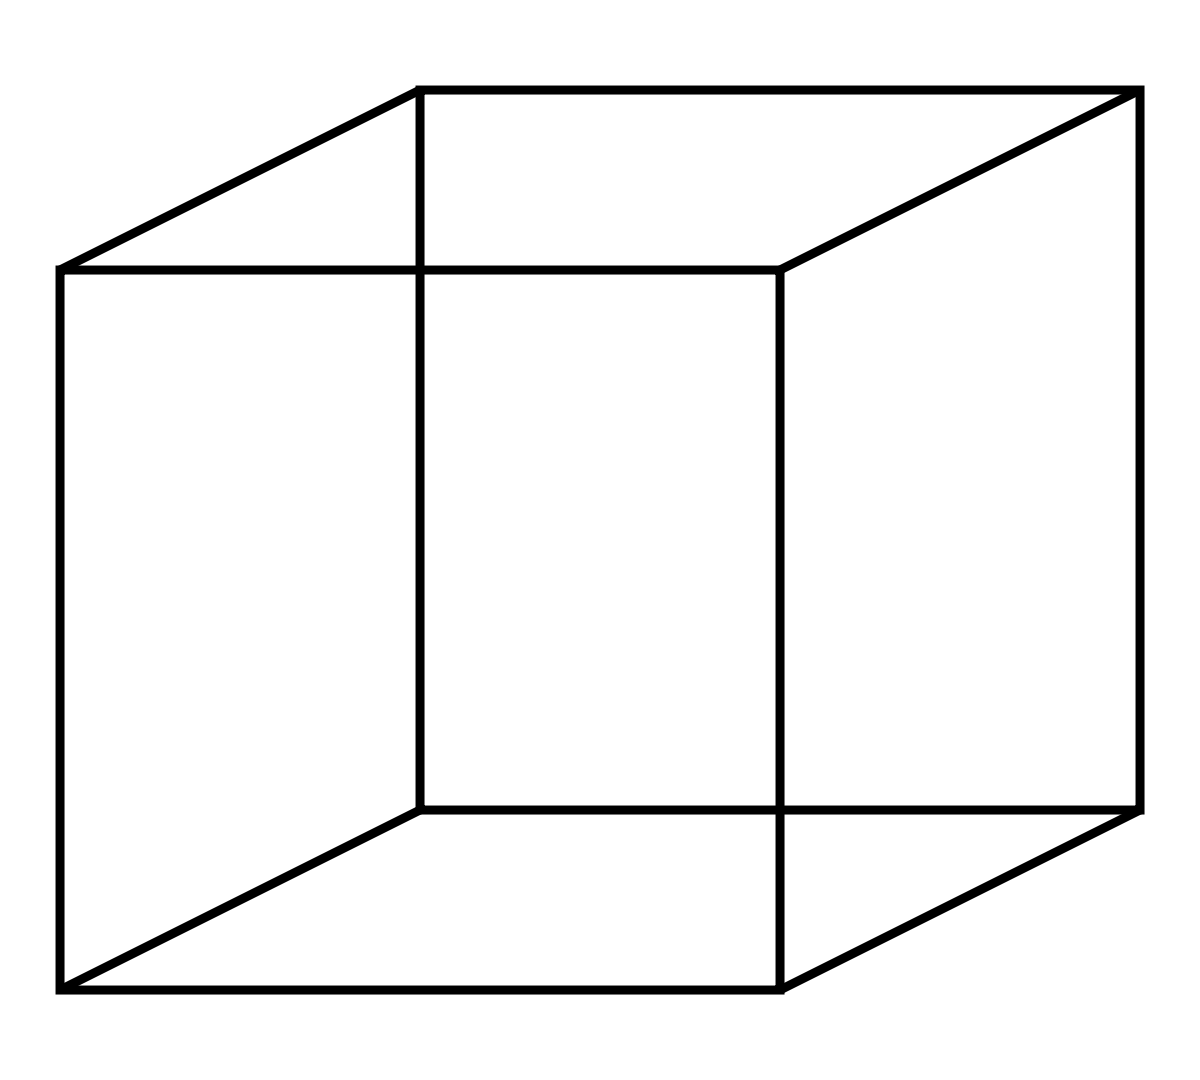
\includegraphics[width=\textwidth]{figs/cubo_necker}
	\end{subfigure}
	\qquad\qquad\qquad
	\begin{subfigure}[]{0.3\textwidth}
		\caption{A imagem se assemelha tanto com um cão de frente quanto um homem de costas}
		\label{fig:cao_homem}
		
\includegraphics[width=0.8\textwidth]{figs/cao_homem}
	\end{subfigure}
	%TODO: citação
\end{figure}
Quando são simuladas as conexões entre um grupo de neurônios, é conveniente considerar a atividade média deles, ou seja, a taxa de disparo dentre eles, e esse conjunto de neurônios é chamado de \textbf{unidade}. No caso da bi-estabilidade, por exemplo, duas unidades rivalizam entre si, conforme mostrado na Figura~\ref{fig:unidadesdecisao}. No exemplo, $s_1$ e $s_2$ são os estímulos, diferenciados apenas pela eventual presença de ruído. As saídas $r_1$ e $r_2$ são as taxas médias de disparo de cada unidade, e cada uma delas também serve como entrada para a mesma, comportamento chamado de \textbf{\textit{feedback} recorrente}. Além disso, há uma interconexão entre as unidades, com a saída de uma se tornando entrada de outra. Tanto as entradas quando as conexões recorrentes são excitatórias (representadas pelos triângulos no topo das unidades), reforçando a taxa de disparo, enquanto as interconexões são inibitórias (representadas pelos círculos pretos). $W^{EE}$ e $W^{IE}$ são as forças das conexões, com o $EE$ indicando a conexão excitatória e $IE$ a inibitória, e $s^E$ e $s^I$ são a fração de canais sinápticos excitatórios e inibitórios, respectivamente, que estão abertos, e são função da taxa de disparos. Além do ruído na entrada, pode ocorrer ruído dentro das unidades, e a presença de ambos pode induzir às transições entre estados bi-estáveis.
% indicar o estímulo
%\begin{figure}[htb!]
%	\centering
%	\caption[Unidades de disparo com \textit{feedback} recorrente]{Unidades de disparo com \textit{feedback} recorrente. A atividade média dos neurônios é simulada, e a saída da unidade também serve como entrada para a mesma. A força da conexão recorrente é excitatória, reforçando a taxa de disparos}
%	\label{fig:feedbackrecorrente}
%	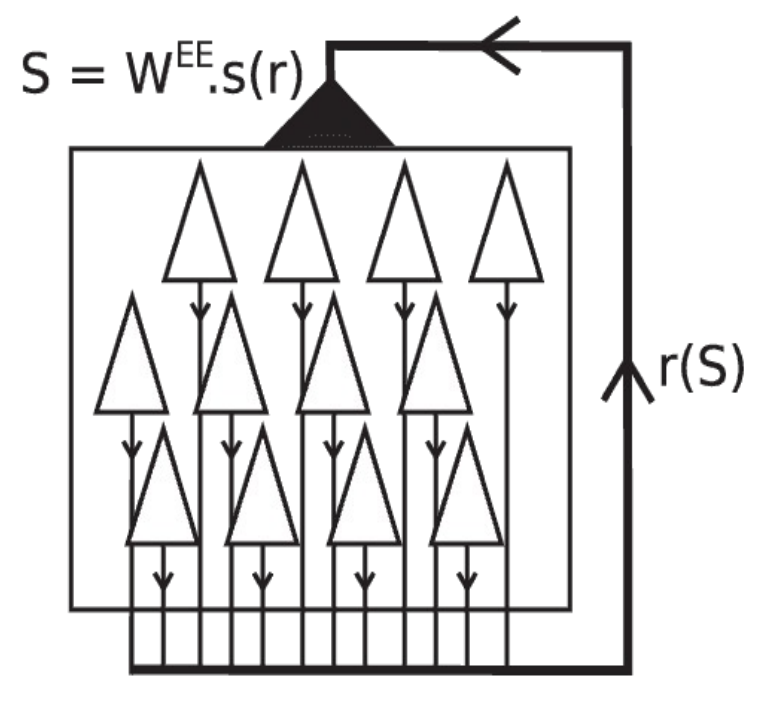
\includegraphics[width=0.45\linewidth]{figs/feedback_recorrente}
%\end{figure}
%sendo $r(S)$ a taxa média de disparos dos neurônios da unidade, que é função da entrada sináptica total, $S$, da fração de canais sinápticos abertos, $s(r)$, variável entre 0 e 1, multiplicado pela força de feedback, $W^{EE}$, o $EE$ indicando que é um feedback excitatório.
% ligar ambas as figuras
%\begin{figure}[ht!]
%	\centering
%	\caption[Unidade com feedback recorrente que determina a estabilidade de um circuito]{Unidade com feedback recorrente que determina a estabilidade de um circuito. A taxa de disparo da unidade é uma função sigmoidal, a linha contínua na direita, e o feedback é representado pela linha tracejada. Na direita, a dinâmica da taxa de disparos em função do tempo, com um pulso de entrada entre 0,5 e 0,55 segundos (a região cinza). O feedback, nesse caso, é médio ($W^{EE}=0.6$), onde taxas baixas e altas de estado são estáveis, causando uma transição entre os estados do sistema}
%	\label{fig:biestavel}
%	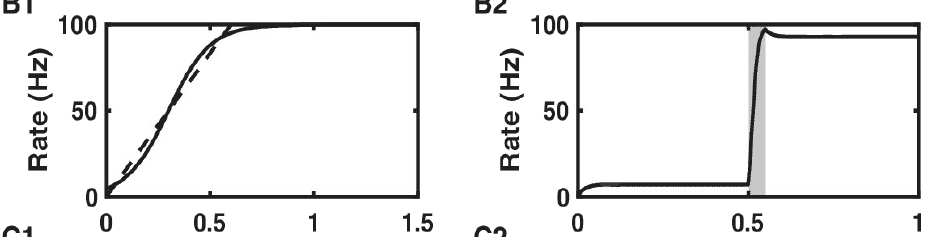
\includegraphics[width=0.7\linewidth]{figs/biestavel}
%\end{figure}


\begin{figure}[tb]
	\centering
	\caption[Unidades de decisão com feedback recorrente e interconexão]{Unidades de decisão com feedback recorrente e interconexão}
	\label{fig:unidadesdecisao}
	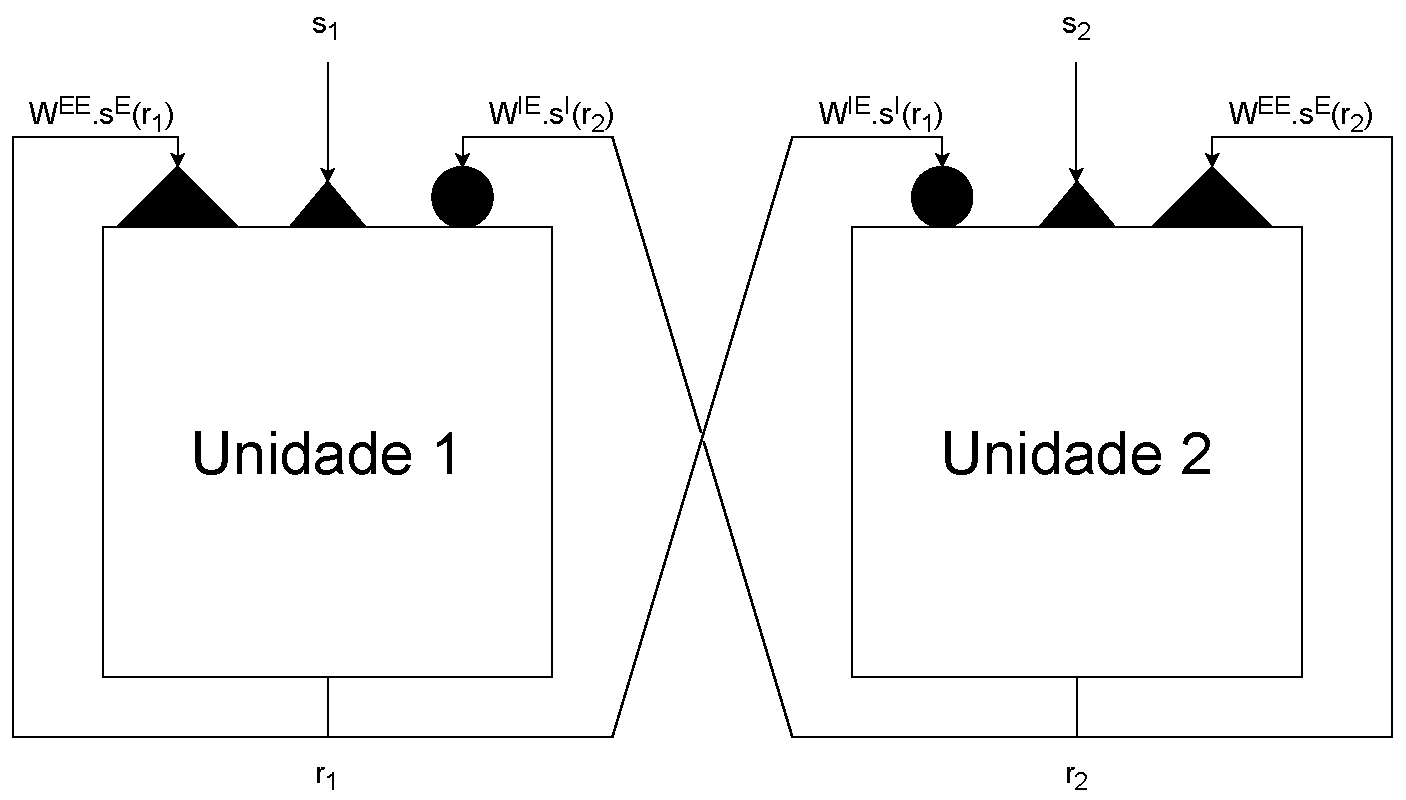
\includegraphics[width=0.7\linewidth]{figs/unidades_decisao}
	%TODO: referência
\end{figure}

%\begin{figure}[htb!]
%	\centering
%	\caption[Transições induzidas por ruído]{Transições induzidas por ruído geram intinerância entre dois estados atratores, explicando alternância perceptual. Em (a), três \textit{trials} separados indicando alteração entre os estados, onde a atividade de uma unidade domina sobre a outra. Em (b), a média das atividades ao longo de 10 \textit{trials} (promediação)}
%	\label{fig:noiseinducedtransitions}
%	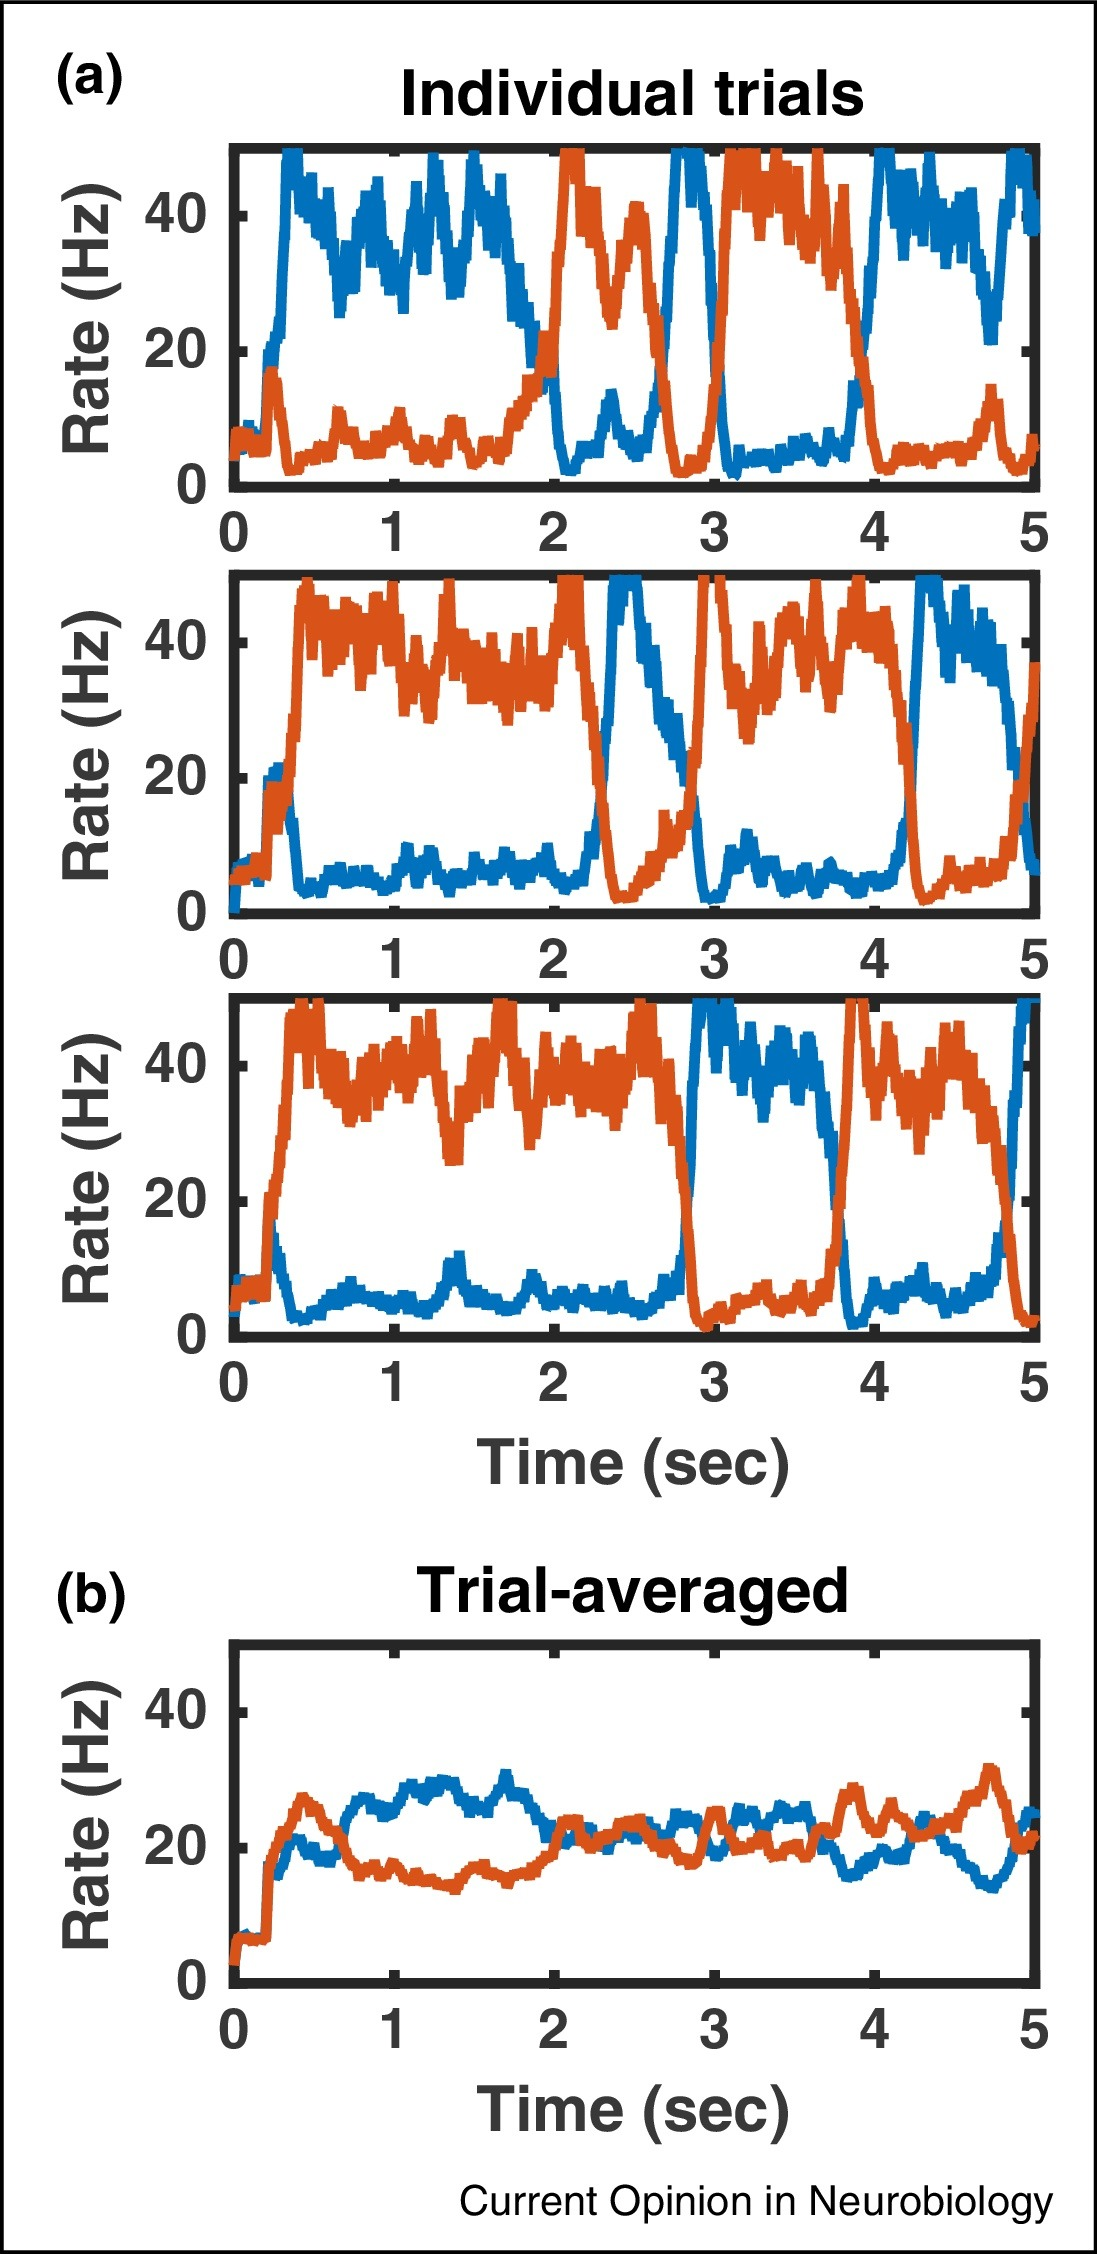
\includegraphics[width=0.35\linewidth]{figs/noise_induced_transitions}
%\end{figure}

\subsection{Circuitos de multi-estabilidade}
Um circuito conhecido de multi-estabilidade é o \textbf{gerador de padrão central} (\textit{central pattern generator}, CPG), que são circuitos neurais que podem reproduzir padrões rítmicos de atividade neuronal sem receber entradas rítmicas.
%TODO: citação Ijspeert
Eles são fundamentais, dentre outras coisas, para circuitos neurais associados à locomoção.

\begin{figure}[tb]
	\centering
	\caption[Gerador de padrão central de duas unidades]{Gerador de padrão central de duas unidades}
	\label{fig:cpg}
	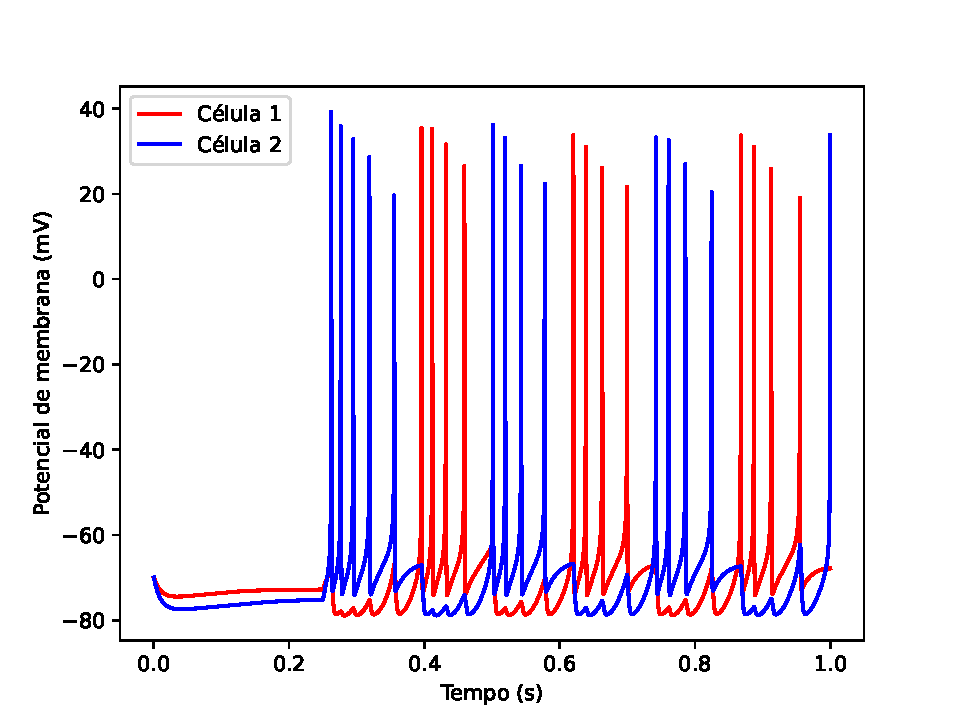
\includegraphics[width=0.7\linewidth]{figs/cpg}
	%TODO: referência
\end{figure}
Um exemplo do seu comportamento é exibido na Figura~\ref{fig:cpg}. Nela, são exibidas as curvas do potencial de membrana de membrana de duas unidades, conectadas como mostrado anteriormente, e com um pulso de corrente aplicado por volta de $0,25\ s$. É possível observar que, quando a célula 1 é ativada (representado pelo disparo dos potenciais de ação), a célula 2 é inibida. O contrário também ocorre, com a célula 1 sendo inibida com a ativação da célula 2, alternando entre qual das unidades dispara durante um intervalo de tempo. Não há o disparo simultâneo das duas células. Um correlato dessa atividade com a locomoção é o movimento das duas pernas humanas. Se associarmos cada perna com uma unidade, hora uma delas está em movimento (uma célula ativada), hora é a outra, alternando ao longo do tempo. Circuitos geradores de padrão central são bastante empregados no projeto de locomoção de robôs articulados.
%TODO: citação Ijspeert

Outros circuitos conhecidos de multi-estabilidade são os de tomada de decisão. Esses circuitos acumulam informações sensoriais ao longo do tempo até que uma decisão possa ser tomada. A computação da informação pode ser feita simplesmente integrando a atividade neural ao longo do tempo,
%TODO: citação cain
como pode ser visto na Figura~\ref{fig:tomadadecisao}. Neste exemplo, um estímulo é aplicado simultaneamente (instante $0\ s$) em duas unidades, também conectadas como acima, que acumulam as evidências desse estímulo ao longo do tempo, alterando a taxa de disparo média das unidades. Neste caso, a decisão tomada, ou seja, a unidade escolhida, é a que atingir primeiro um determinado limiar, definido como a taxa de disparo de $40\ Hz$. A unidade 1 (em azul) foi a vencedora.
\begin{figure}[tb]
	\centering
	\caption[Circuito de tomada de decisão]{Circuito de tomada de decisão}
	\label{fig:tomadadecisao}
	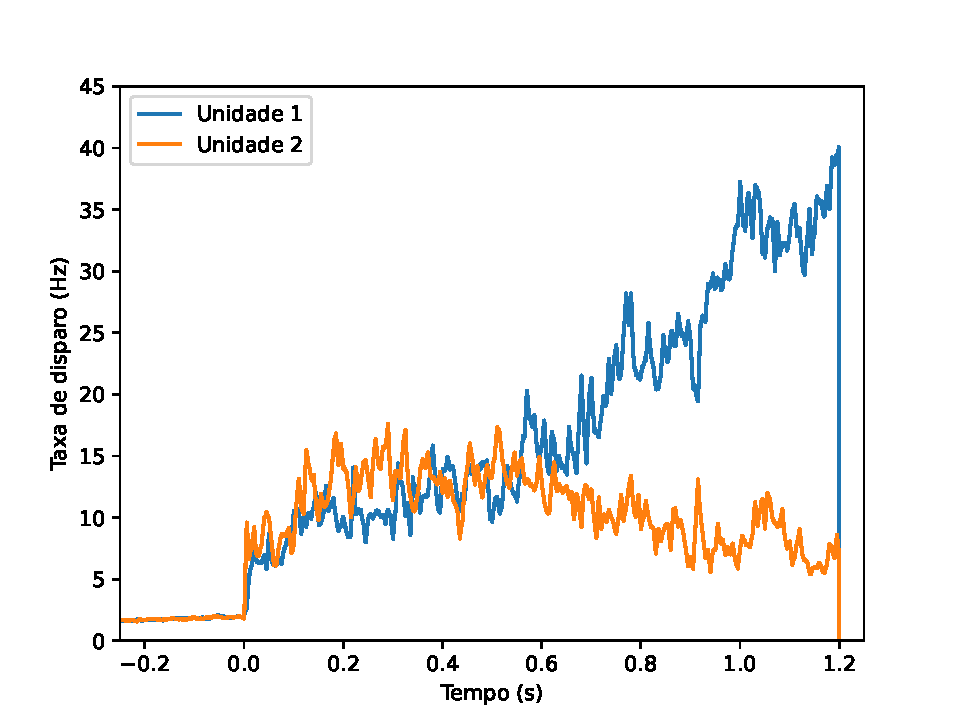
\includegraphics[width=0.7\linewidth]{figs/tomada_decisao}
	%TODO: referência
\end{figure}


\section{Aprendizado e plasticidade de longa duração}\label{sec:aprendizado}

A plasticidade é a capacidade do cérebro de se adaptar, tanto estrutural quanto funcionalmente, em resposta à estímulos externos.
%TODO: citação mateos-aparicio the impact
O termo se torno bastante conhecido principalmente devido à chamada \textbf{Regra de Hebb}, que diz que se um neurônio A excita um neurônio B repetidas vezes, contribuindo para o disparo deste, então a sinapse entre os dois deve ser fortalecida.
%TODO: citação hebb the organization
Diferentemente das alterações de curta duração mostradas na Seção~\ref{subsec:sinapses_dinamicas}, as mudanças das forças de conexões neuronais da plasticidade sináptica persistem por longos períodos de tempo. Um exemplo é o conceito de \textbf{potencialização de longa duração} (\textit{long-term potentiation, LTP, em inglês}), que se trata de um crescimento da força de conexão sináptica que duram por algumas dezenas de minutos.
%TODO: citação bliss long-lasting
Do mesmo modo, há a \textbf{depressão de longa duração} (\textit{long-term depression, LTD, em inglês}), que é a diminuição da força de conexão por um longo período de tempo.
%TODO: citação bear long-term
A regra de plasticidade mais simples é dada pela equação abaixo:
\begin{equation}\label{eq:regra_hebb}
	\tau_w\dfrac{\mathrm{d}\mathbf{w}}{\mathrm{d}t}=v\mathbf{u}
\end{equation}
onde $\tau_w$ é uma constante de tempo que controla a taxa em que os pesos se atualizam, $w$ é o vetor de pesos sinápticos, $v$ é a atividade do neurônio pós-sináptico e $u$ o vetor de atividades dos neurônios pré-sinápticos.

Na versão simplificada de plasticidade exibida acima, tanto a atividade do neurônio pré-sináptico quanto a do pós aumentam a força da conexão. Na prática, porém, há uma espécie de competição entre diferentes sinapses, que pode ser observada na chamada \textbf{plasticidade dependente do tempo de disparo} (\textit{spike-timing dependent plasticity}, STDP, em inglês), que depende do tempo relativo do disparo das células pré e pós-sinápticas, como exibido na Figura~\ref{fig:stdp}.
%TODO: citação song competitive
\begin{figure}[tb]
	\centering
	\caption[Plasticidade dependente do tempo de disparo (STDP)]{Plasticidade dependente do tempo de disparo (STDP)}
	\label{fig:stdp}
	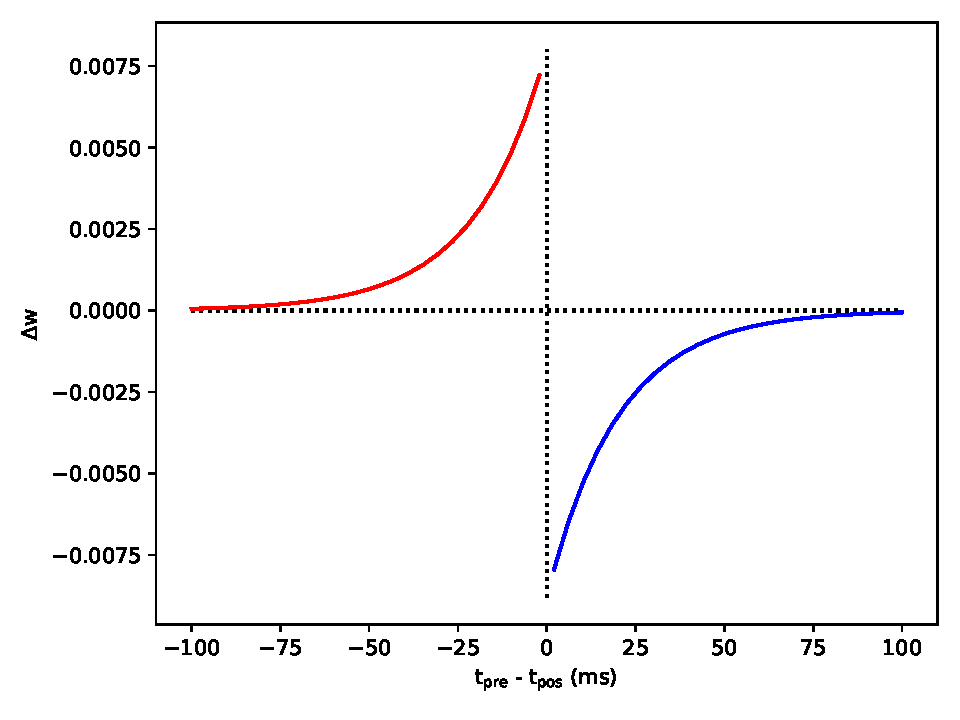
\includegraphics[width=0.7\linewidth]{figs/stdp}
	\legend{Fonte: o autor (\the\year)}
	%TODO: ajustar rótulo da ordenada
\end{figure}
Na abscissa é apresentada a diferença de tempo entre os disparos dos neurônios pré e pós-sinápticos. 0~(zero) significa que ambos disparam ao mesmo tempo, valores negativos estão associados ao neurônio pré-sináptico disparando primeiro, e valores positivos ao disparo do neurônio pós-sináptico primeiro. Na primeira situação, com o pré seguido do pós (curva em vermelho), a atividade resulta em uma potencialização de longa duração, com a diferença de peso sendo maior proporcionalmente à diminuição do tempo entre os disparos, até próximo de 0~(zero), enquanto na situação onde o pós-sináptico dispara primeiro (curva em azul), a atividade resulta em uma depressão de longa duração, também com a diferença de peso aumentando proporcionalmente com a diminuição da diferença de tempo entre os disparos.

A modelagem da STDP é dada pela equação abaixo:
%TODO: citação song competitive
\begin{equation}\label{eq:stdp}
	\Delta_w=\begin{cases}
		A_+\exp(\Delta t/\tau_+)\quad\text{se }\Delta t<0\\
		-A_-\exp(-\Delta t/\tau_-)\quad\text{se }\Delta t\geq0
	\end{cases}
\end{equation}
sendo $A_+$ e $A_-$ os valores máximos de modificação sináptica, ambos com valor positivo e o máximo próximo de $\Delta_t=0$. $\tau_+$ e $\tau_-$ são as faixas de intervalo entre disparo das células pré para pós-sinápticas. A STDP é uma das bases de aprendizado de diversos algoritmos de aprendizado de máquina, que serão apresentados no Capítulo seguinte.

%\subsection{Redes Hopfield}
%
%\section{Caos e criticalidade}\label{sec:caos}
%% colocar introdução
%% transição de estados
%% matemática dos estados
%
%\subsection{Nullclines}
%\begin{description}
%	% isóclina de inclinação nula
%	\item[Fase-plano] \textit{Plots} dos eixos das duas variáveis em um sistema de duas equações diferenciais ordinárias. Mostram os pontos fixos, \textit{nullclines} e trajetórias das variáveis ao longo do tempo
%	\item[\textit{Nullcline} (Isóclina de inclinação nula)] Curvas que mostram a dependência de pontos fixos entre as variáveis de um sistema de equações diferenciais ordinárias. Cada equação diferencial gera uma \textit{nullcline}, e as interseções entre elas definem os pontos fixos do sistema
%	%\item[Quebra do anôdo] Um disparo no potencial de membrana que ocorre logo após uma hiperpolarização
%	\item[Pontos fixos] Pares de valores onde o sistema não se altera (o lado direito da equação diferencial ordinária é igual a 0)
%\end{description}
%
%% exemplo lotka-volterra
%\begin{figure}[htb!]
%	\centering
%	\caption{\textit{Nullclines} em sistemas de Lotka-Volterra}
%	\label{fig:nullclineslotkavolterra}
%	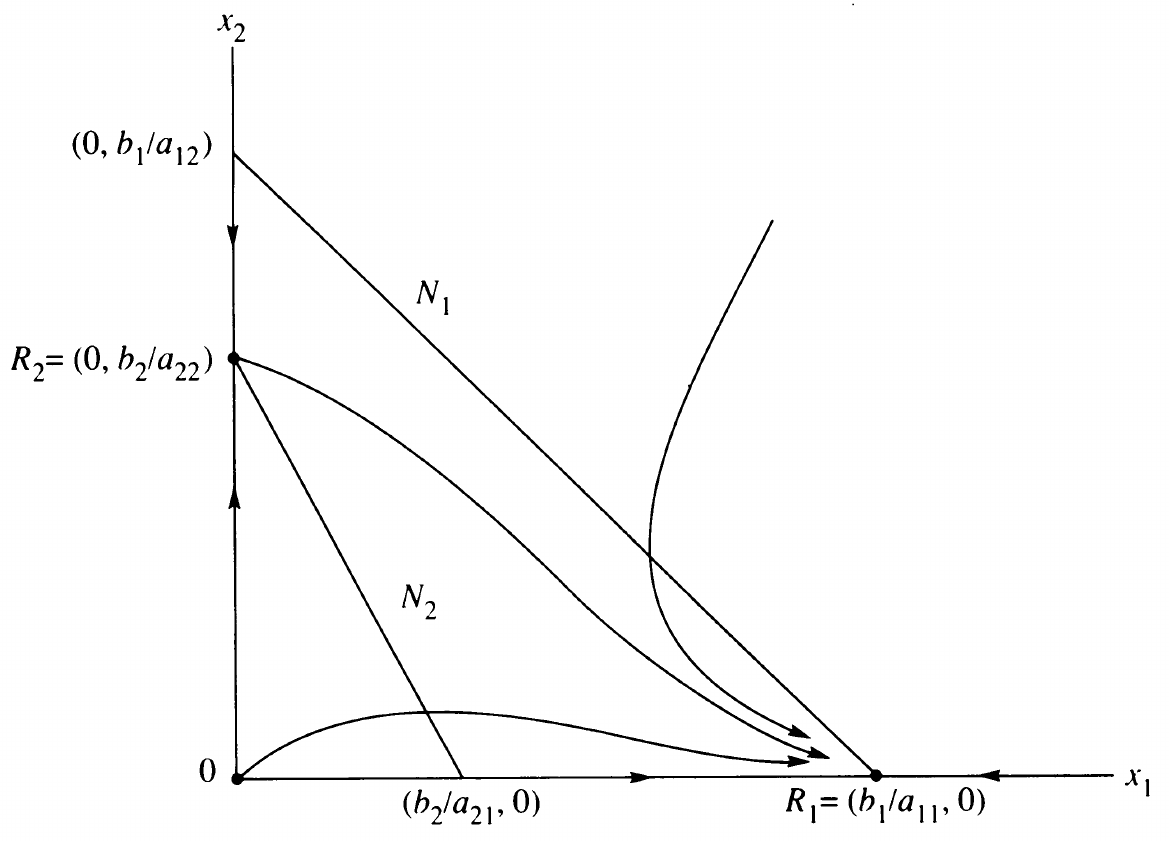
\includegraphics[width=0.7\linewidth]{figs/nullclines_lotka_volterra}\\
%	\small{Fonte: \cite{zeeman_extinction_1995}}
%\end{figure}
%
%% exemplo fitz-hugh nagumo
%\begin{figure}[htb!]
%	\centering
%	\caption{Plano de fase e estados fisiológicos no modelo FitzHugh-Nagumo}
%	\label{fig:fitzhugh}
%	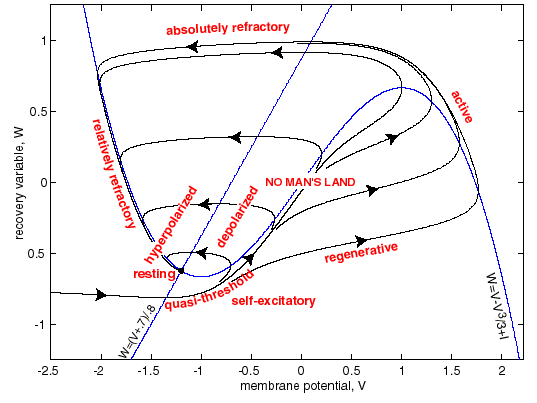
\includegraphics[width=0.7\linewidth]{figs/fitzhugh}\\
%	\small{Fonte: Scholarpedia}
%\end{figure}
%
%% exemplo izhikevich
%% exemplo livro (sistemas bi-estáveis)
%\begin{figure}[htb!]
%	\centering
%	\caption[\textit{Nullclines} mostrando pontos fixos de sistemas bi-estáveis]{\textit{Nullclines} mostrando pontos fixos de sistemas bi-estáveis. A linha pontilhada é para $r_2$, e a contínua é para $r_1$. Os pontos fixos, onde as linhas se interceptam, são representados pelos círculos. Os sólidos são pontos estáveis, enquanto os abertos são instáveis.}
%	\label{fig:nullcline}
%	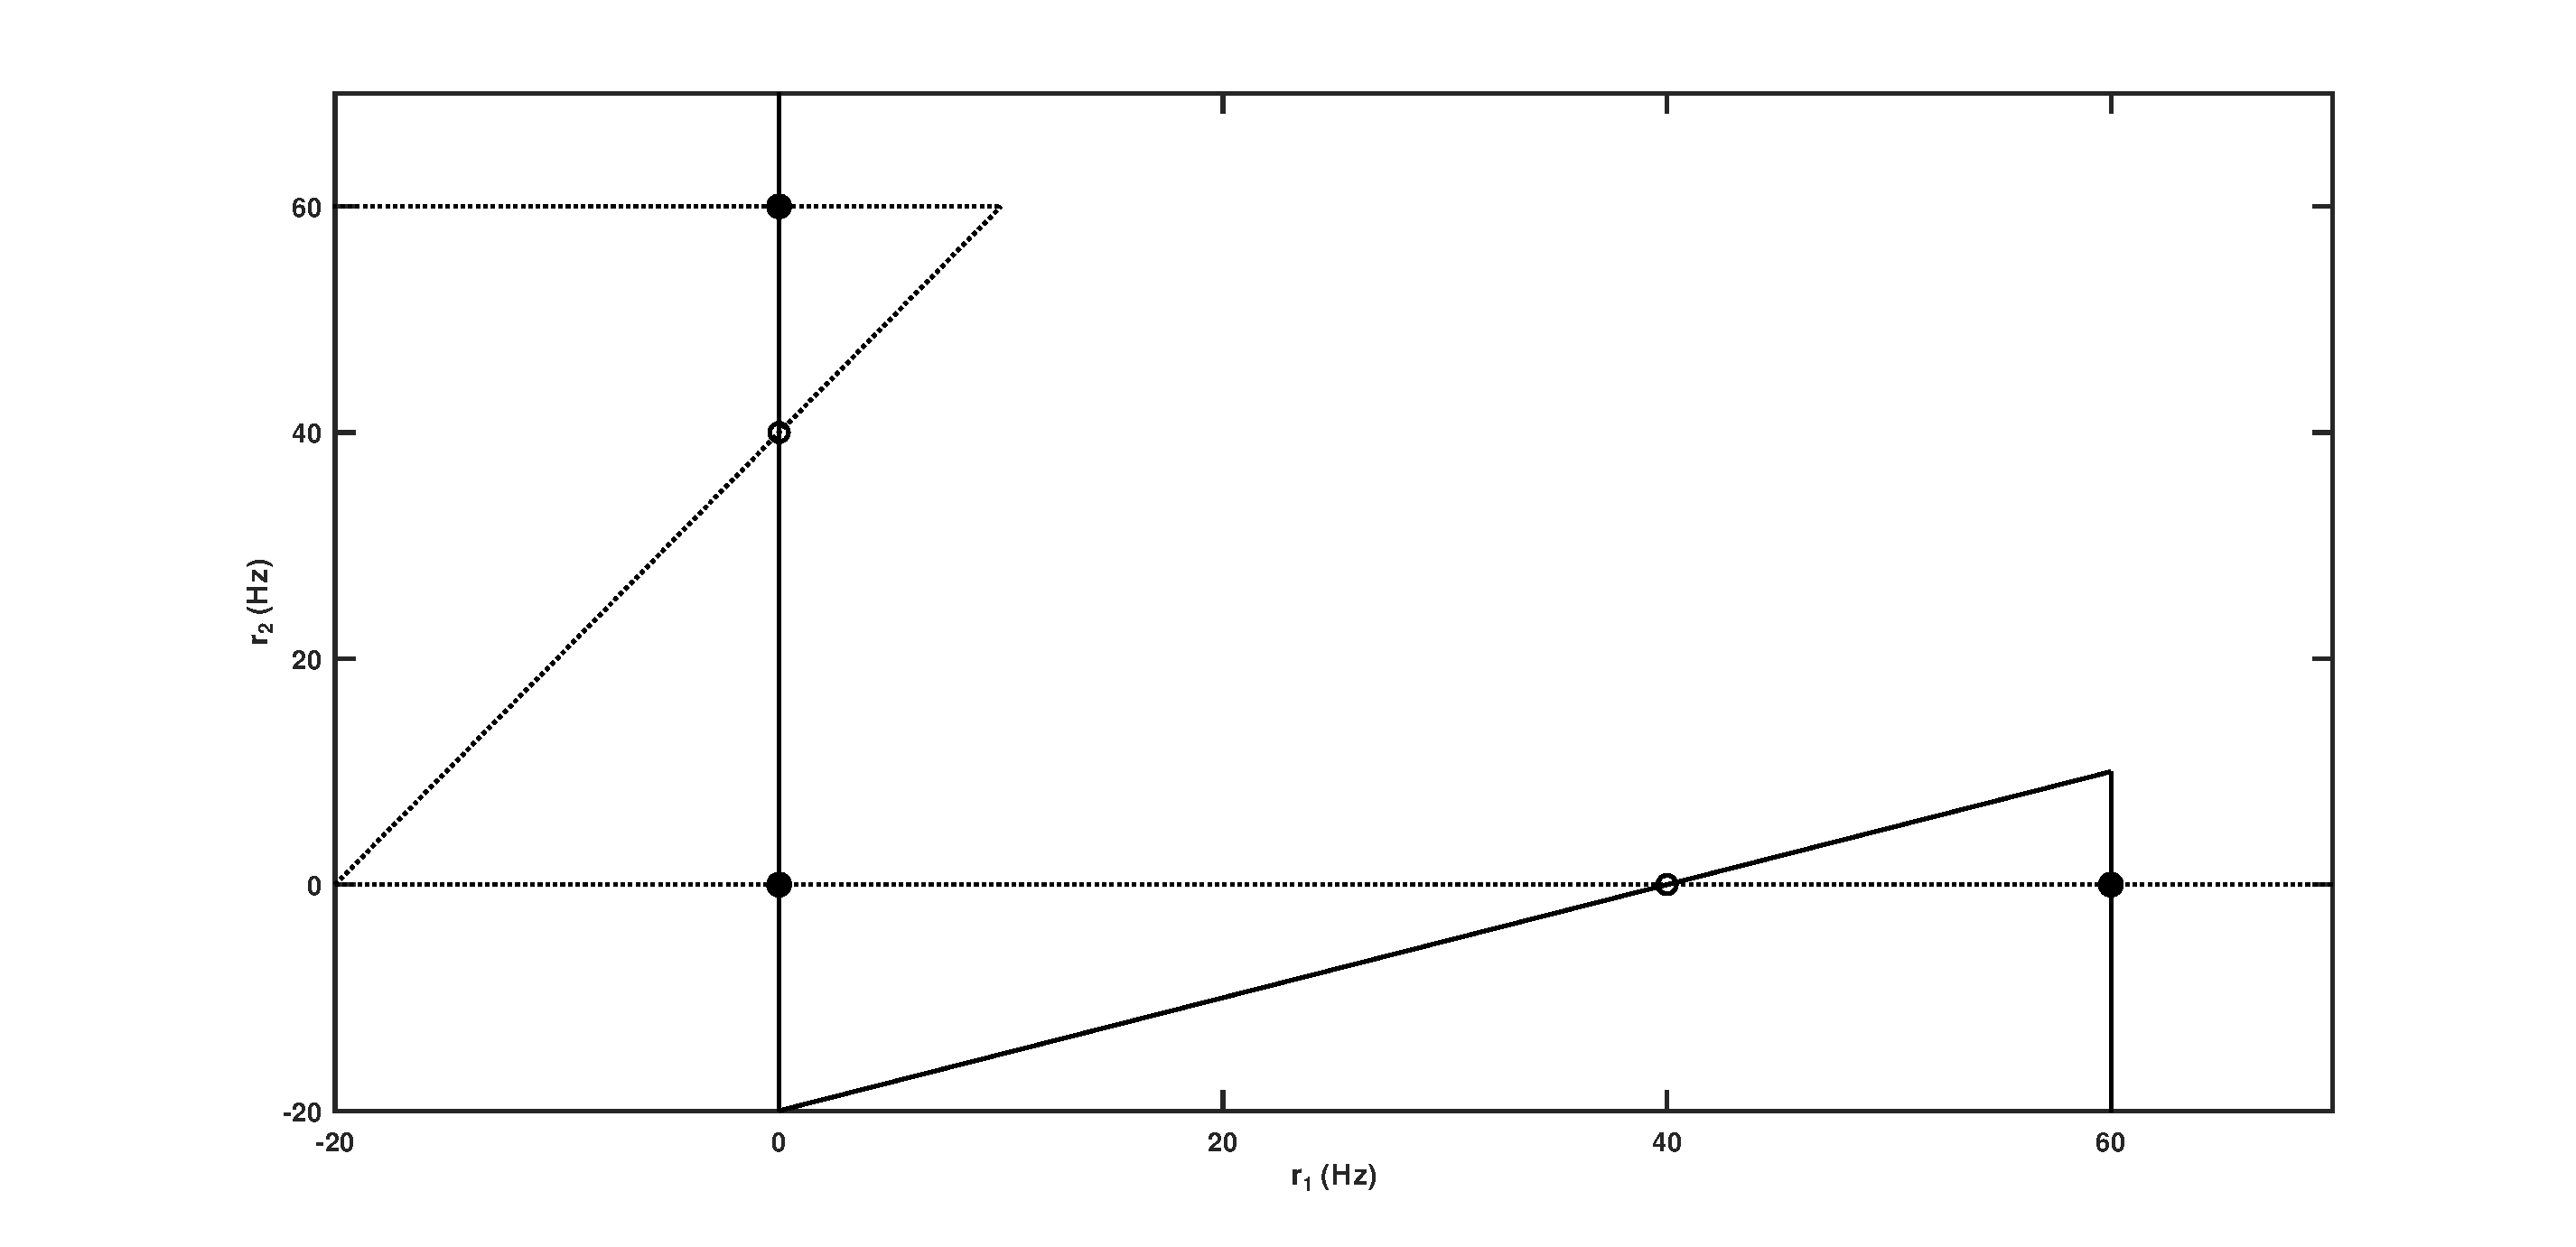
\includegraphics[width=0.9\linewidth]{figs/nullcline}\\
%	\small{Fonte: adaptado de \cite{miller_introductory_2018}}
%\end{figure}
%
%
%\subsubsection{Múltiplos atratores}
%\begin{itemize}
%	\item Alterações para mais de dois estados perceptuais
%	\item Podem ser representados usando modelos ocultos de Markov (HMM, \textit{Hidden Markov Models})
%	\item Na Figura~\ref{fig:hmm}, em (b), são mostrados os estados discretos que o HMM pode assumir nesse caso (círculos coloridos), com as matrizes de probabilidades de transição entre estados por unidade (a espessura das setas).
%	\item Cada estado é definido pela probabilidade de emissão de um padrão particular em um intervalo de tempo (histogramas dentro dos círculos)
%\end{itemize}
%
%\begin{figure}[htb!]
%	\centering
%	\caption[Modelos ocultos de Markov]{Modelos ocultos de Markov. Em (a), os conjuntos de trens de disparo de potenciais de ação. Em (b), os estados discretos que o HMM assume. Em (c), as probabilidades a posteori para cada estado}
%	\label{fig:hmm}
%	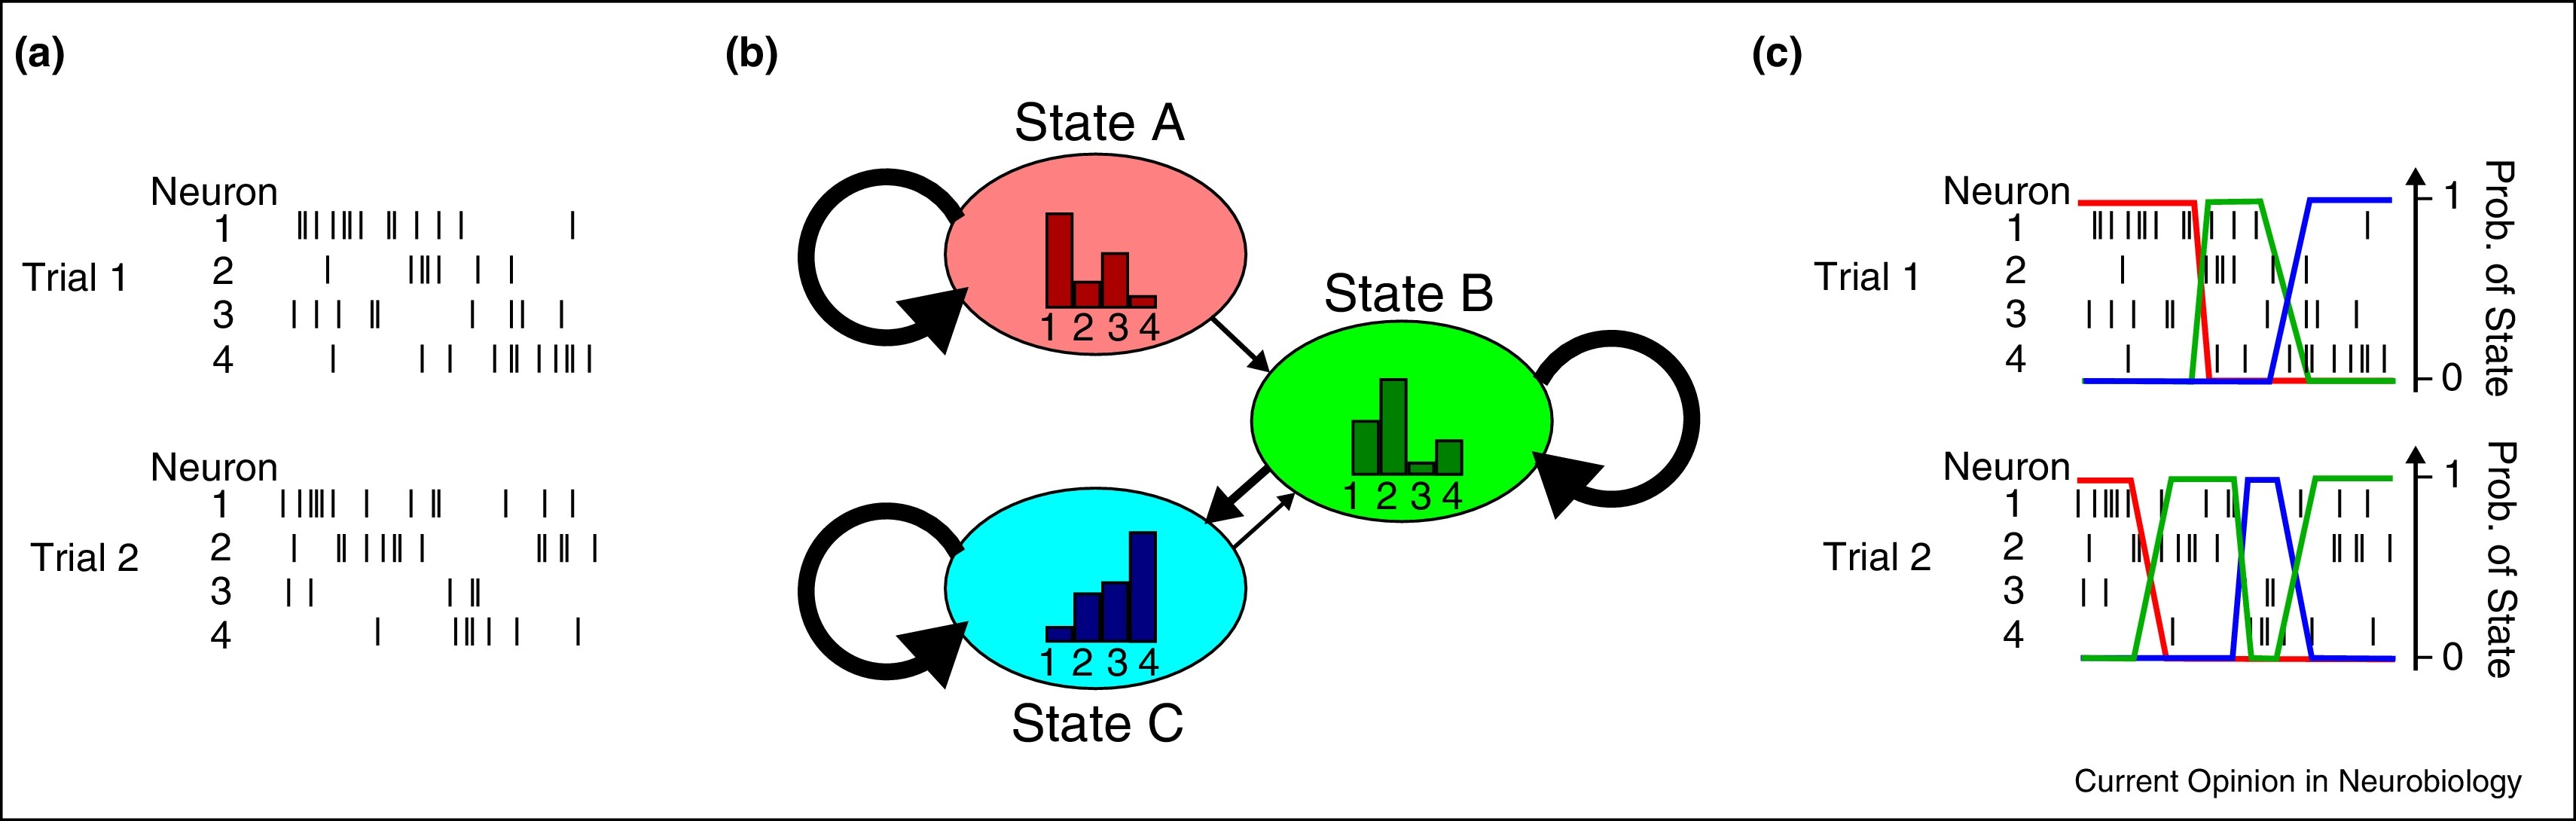
\includegraphics[width=0.8\linewidth]{figs/hmm}
%\end{figure}
%
%
%\subsection{Caos}
%\begin{itemize}
%	\item A \textbf{teoria do caos} é um ramo da matemática que lida com sistemas dinâmicos não lineares, ou seja, a interação dos componentes do sistema não é somente a adição desses componentes individualmente, devido a existência de efeitos multiplicativos ou de \textit{feedback}
%	\item Sistemas caóticos podem ter poucas partes e seguirem regras bem simples, porém possuem uma sensibilidade bem grande às condições iniciais, onde o impacto de um pequeno efeito pode crescer exponencialmente ao longo do tempo
%	\item A dinâmica não-linear de sistemas com caos facilita a habilidade de adaptação presente em sistemas neuronais, causando transições de um padrão de comportamento para outro quando o ambiente é alterado e, consequentemente, criando uma rica variedade de padrões
%	\item Sistemas operam na \textbf{beira do caos} quando, para um mesmo conjunto de parâmetros, se ajustados em uma direção tornam o sistema caótico, enquanto que se ajustados em outra direção fazem com que o sistema apresente estados estáveis
%	\item O conjunto de parâmetros, na condição de beira do caos, pode ser chamado de crítico, com o sistema podendo exibir \textbf{criticalidade}, uma propriedade dos sistemas onde uma pequena alteração do sistema em um local pode tanto ter um efeito local quanto se propagar e alterar o sistema como um todo
%	\item Acredita-se que sistemas em criticalidade possuem melhores capacidades de processamento de informação e otimização de memória, inspirando a hipótese da criticalidade, proposição onde o cérebro opera em um estado crítico, devido às capacidades de computação ótimas associadas precisarem ser evolutivamente selecionadas para isso
%	\item A ideia geral de sistemas se auto migrarem para estados críticos através de processos descentralizados é conhecido como \textbf{criticalidade auto-organizável} (SOC, \textit{self-organized criticality})
%	\item Uma cascata de disparos de atividade neuronal que ultrapassa um limiar em intervalos de tempo seguidos é chamado de \textbf{avalanche} (Fig.~\ref*{fig:sandpile})
%	\item Exemplos de sistemas que podem exibir comportamento caótico incluem o modelo de neurônio de Izhikevich (já visto) e a equação do mapa logístico (tutorial), dada por $x_{t+1}=rx_t(1-x_t)$, e que representa um modelo discreto de crescimento populacional, sendo $x_t$ a taxa de população no tempo $t$ e $r$ a taxa de crescimento
%\end{itemize}
%
%\begin{figure}[htb!]
%	\centering
%	\caption{Modelo de pilha de areia}
%	\label{fig:sandpile}
%	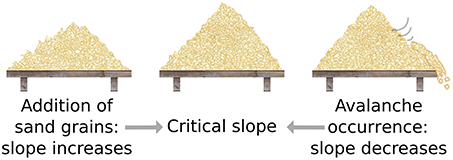
\includegraphics[width=0.7\linewidth]{figs/sandpile}
%\end{figure}

%\subsection{Coeficiente de Lypunov}

%\subsection{Avalanches}
